\chapter{Revisão Teórica} \label{revisao}

Esta seção visa oferecer os conceitos necessários para o completo entendimento desse trabalho. Inicialmente, serão apresentados os conceitos relacionados a classificação de satélites, o padrão \textit{CubeSat}, alguns conceitos de eletrônica e, por fim, um histórico das missões anteriores com enfoque nos sistemas de potência utilizados.

\section{Nanossatélites}\label{nanosats_revision}
A classificação mais utilizada para satélites é com relação a sua massa. Na figura abaixo, podemos ver as categorias utilizadas nessa classificação e alguns exemplos de artefatos já lançados. Observe que os nanossatélites se encontram na faixa de 1 até 10 kg.

\noindent
\begin{minipage}{\linewidth}
\makebox[\linewidth]{
    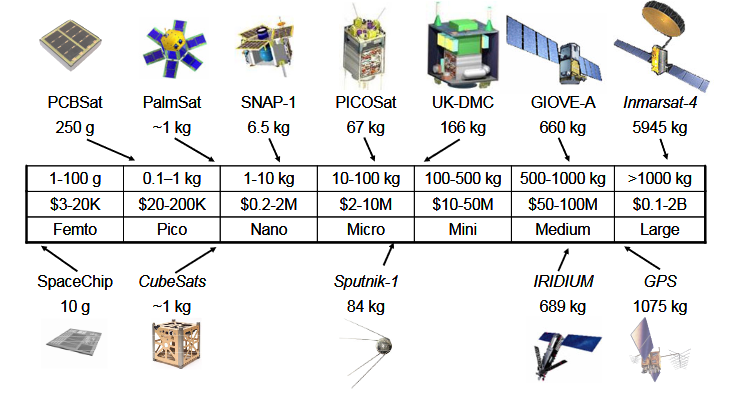
\includegraphics[keepaspectratio=true, scale=0.7]{imagens/Satellite-mass-classification.png}}
\label{mass_classification_fig}
\captionof{figure}{Classificação de satélites, com alguns exemplos. Fonte: \cite{barnhart_ref}.}
\end{minipage}

 Os principais responsáveis por essa redução de massa são a miniaturização dos circuitos integrados e as padronizações das estruturas de lançamento, como no padrão \textit{CubeSat}. Os nanossatélites são amplamente utilizados nas atividades de ensino, pois permitem um ciclo completo de uma missão espacial mantendo um custo baixo, principalmente devido ao uso de peças comerciais.\cite{barnhart_ref}

\section{\textit{CubeSat}}\label{cubesat_revision}

O padrão \textit{CubeSat} foi um dos grandes responsáveis pela popularização da categoria de nanossatélites, como se vê no gráfico abaixo, que mostra o número de lançamentos desse tipo por ano.\cite{cubesats_cgee}.

\noindent
\begin{minipage}{\linewidth}
\makebox[\linewidth]{
    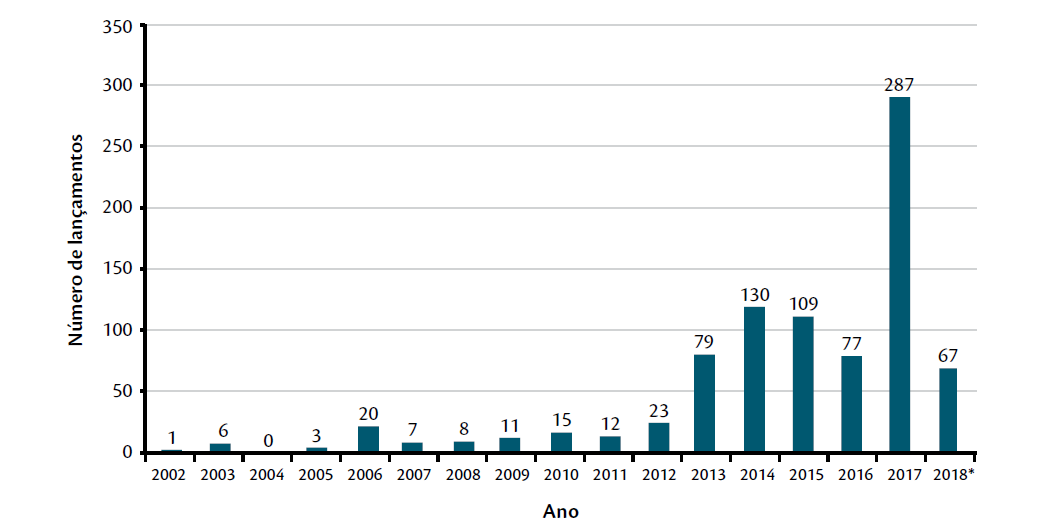
\includegraphics[keepaspectratio=true, scale=0.6]{imagens/cubesat-launches-count.png}}
\captionof{figure}{Distribuição do número de \textit{CubeSats} pelo ano de lançamento. Fonte: \cite{cubesats_cgee}.}
\label{cubesat_launches_fig}
\end{minipage}

O modelo \textit{CubeSat} foi proposto em 1999 por Jordi Puig-Suari, da \textit{California Polytechnic State University}, e Bob Twiggs, da \textit{Stanford University}. O objetivo era um modelo de satélite de pequeno porte que segue um padrão mais simples, o intuito deles era fornecer aos alunos de ambas universidades a oportunidade de  participar de um projeto espacial completo, incluindo todas as fases, desde a construção, testes e operação do artefato, que manteria características similares aos satélites maiores. O termo é um acrônimo entre as palavras \textit{cube} (em inglês, cubo) acrescida das três primeiras letras da palavra satélite.

Normalmente, as missões com \textit{CubeSats} tem um risco técnico mais elevado, em parte devido ao uso de componentes não \textit{"space qualified"}, porém oferecem em troca uma implementação mais rápida, aplicações mais inovadoras, custos menores ou um conjunto desses elementos.

As principais características dos \textit{CubeSats} são as seguintes:
\begin{itemize}
    \item compostos por unidades cúbicas padronizadas (1U) de tamanho 10x10x10 cm, conforme mostrado na figura \ref{cubesat_configs_fig};
    \item uso de sistemas padronizados de ejeção em órbita, denominados, P-POD (do inglês, \textit{Poly Picosatellite Orbital Deployer}) ou SSPL (do inglês, \textit{Space Shuttle Picosatellite Launcher}). Esses sistemas são capazes de liberar diversos satélites pela mesma interface;
    \item componentes COTS nos sistemas de bordo.
\end{itemize}

\noindent
\begin{minipage}{\linewidth}
\makebox[\linewidth]{
    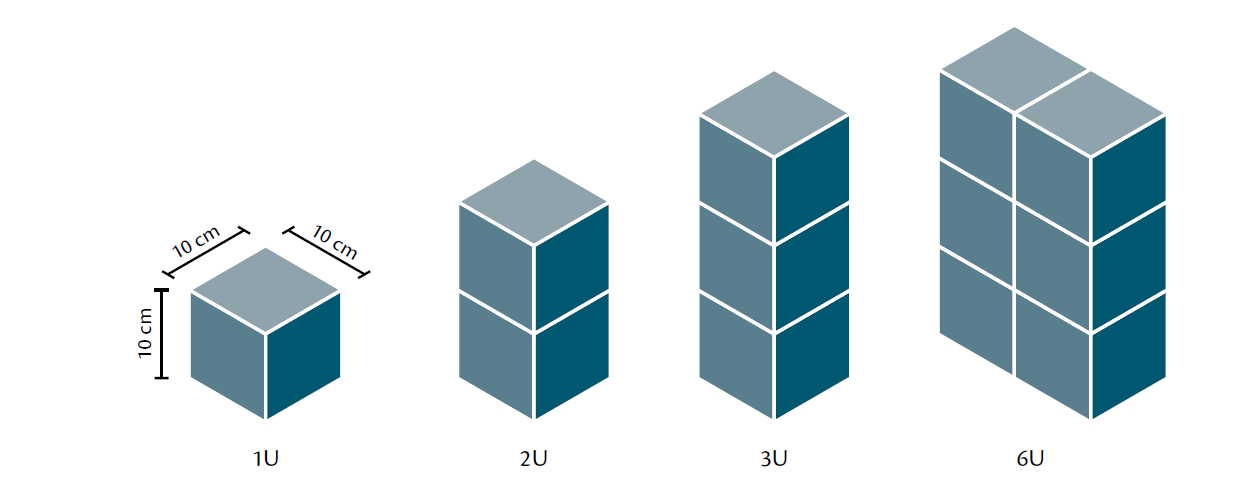
\includegraphics[keepaspectratio=true, scale=0.6]{imagens/cubesats-configs.png}}
\captionof{figure}{Algumas configurações de \textit{CubeSats}. Fonte: \cite{cubesats_cgee}.}
\label{cubesat_configs_fig}
\end{minipage}

O padrão é descrito em um documento de domínio público\cite{cubesat_specs_rev13}, onde se especifica que uma unidade \textit{CubeSat} ou 1U, tem um volume de 1 litro e carga útil de até 1,3 kg, podendo combinar várias unidades dessas para compor satélites maiores (2U, 3U, 6U ou 12U, por exemplo). A figura \ref{cubesat1U_dimensions_fig} mostra as especificações mecânicas da unidade \textit{CubeSat}.

\noindent
\begin{minipage}{\linewidth}
\makebox[\linewidth]{
    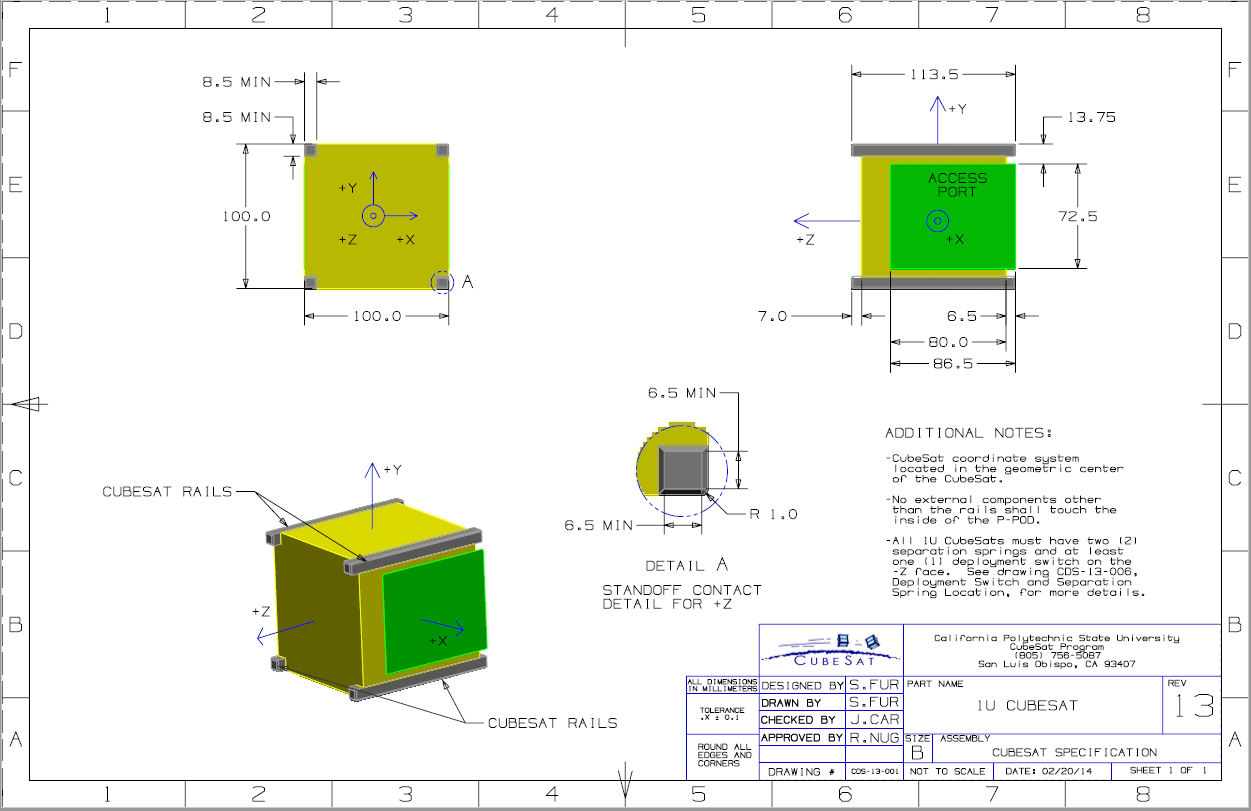
\includegraphics[keepaspectratio=true, scale=0.5]{imagens/Cubesat-diagram.png}}
\captionof{figure}{Especificações de dimensionamento para um \textit{CubeSat} 1U. Fonte: \cite{cubesat_specs_rev13}.}
\label{cubesat1U_dimensions_fig}
\end{minipage}

Quanto aos requisitos elétricos, o padrão apresenta dois requisitos extremamente importantes que são o \textit{Deployment Switch} e o pino \textit{Remove Before Flight} (RBF).

O \textit{Deployment Switch} é uma chave que deve desconectar eletricamente todos os subsistemas, sem exceções, do sistema de potência. Essa chave deve atuar durante todo o tempo que o CubeSat estiver acoplado no P-POD, e esse sinal é recebido dos trilhos do P-POD, conforme figura \ref{cubesat1U_dimensions_fig}.
Por sua vez, o RBF, é um pino que deve cortar toda a alimentação do satélite uma vez que estiver inserido. Ele será removido após o encaixe na base de lançamento P-POD e não deve avançar mais do que 6.5 mm além dos trilhos.

Por esses e outros aspectos, os \textit{CubeSats} trouxeram um aspecto inovador capaz de mudar o paradigma do setor espacial, adequando-o à nova tendência de emprego de pequenos satélites para atender a diferentes tipos de demandas.

\section{Paineis Solares}
Os painéis solares, ou PV\footnote{Photovoltaics - conforme literatura em inglês sobre o assunto}, são dispositivos que utilizam o efeito fotovoltaico para produzir energia elétrica. Nas células solares, a diferença de potencial surge quando um elétron recebe energia suficiente para passar da camada de valência para a camada de condução do material semicondutor.

Diferente dos metais, os semicondutores possuem a camada de valência completamente cheia e a camada de condução completamente vazia, e o salto "\textit{gap}" entre as duas camadas é de 1 eV (elétron-volt). Caso o fóton incidente na placa forneça mais energia do que o necessário para o elétron atravessar o salto, o excesso se transforma em calor, em um efeito conhecido como termalização.

\subsection*{Curva I-V}
A curva I-V\footnote{Curva Corrente x Tensão} é uma das características mais importantes quando se projeta algo com painel solar, pois é necessário conhecer e realizar a previsão de parâmetros importantes como a irradiação solar, temperatura e carga que será atendida. A maioria dos métodos presentes na literatura utiliza a curva I-V para o cálculo desses parâmetros ou então outros métodos de natureza empírica, a seguir vamos usar essa técnica\cite{pv_datasheet} para montar um modelo para as simulações.

\subsection*{Modelo para simulação}
A curva I-V geral de um painel solar é baseada no modelo exponencial \cite{pv_datasheet}:
\begin{equation}
    i = I_{ph} - I_{o}(e^{\frac{v + iR_{s}}{n_{s}V_{t}}}-1) - \frac{v + iR_{s}}{R_{sh}}
\end{equation}
Na equação acima, $V_{t}$ é a tensão térmica da junção P-N.
\begin{equation}
    V_{t} = \frac{AkT_{stc}}{q}
\end{equation}

Com esses parâmetros, forma-se o circuito equivalente, mostrado na figura \ref{PV_equivalent_circuit_fig}, para uma célula solar:

\noindent
\begin{minipage}{\linewidth}
\makebox[\linewidth]{
    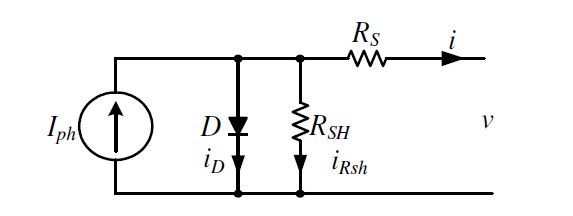
\includegraphics[keepaspectratio=true, scale=0.8]{imagens/PV_eq_circuit.PNG}}
\captionof{figure}{Circuito equivalente para uma célula fotovoltaica, usando o modelo exponencial. Fonte: \cite{pv_datasheet}.}
\label{PV_equivalent_circuit_fig}
\end{minipage}


Os parâmetros do modelo são $I_{ph}$ - Corrente gerada pela célula, $I_{o}$ - Corrente de saturação, $R_{s}$ - Resistência em série da célula, $R_{sh}$ - Resistência em paralelo da célula (shunt) e $A$ - Fator de qualidade do diodo. Além desses parâmetros, $k$ é a constante de Boltzmann, $q$ é a carga do elétron, $n_{s}$ é o número de células conectadas em série, e $T_{stc}$ ($K$) é a temperatura na STC\footnote{STC, sigla para \textit{Standard Test Conditions}, condições de teste para aferir as medidas de caracterização de um painel solar.}.

\section{Conversores DC-DC}\label{converters_revision}
Conversores DC-DC \cite{ti_whitepaper}\cite{power_electronics_hart} são dispositivos eletrônicos capazes de converter uma tensão de entrada em uma tensão diferente e, normalmente, fornecem uma saída regulada. Os conversores do tipo chaveados estão cada vez mais comuns devido a alta eficiência e por permitirem uma flexibilidade de projeto, ou seja, da mesma tensão de saída é possível gerar multiplas tensões de saída de projetos diferentes. Existem quatro topologias de conversões bastante comuns, porém as próximas subseções detalharão brevemente os princípios de funcionamento das topologias necessárias para o entendimento do trabalho que são a \textit{Buck} e a \textit{SEPIC}.

Antes de continuar para as topologias, inicialmente, vamos entender o significado de "ser chaveado". Em um circuito chaveado, existirá um transistor que atuará como chave, ou seja, alterará entre os estados completamente ligado e completamente desligado. Para um transistor do tipo BJT isso significa transicionar entre os estados de corte e saturação, no transistor do tipo MOSFET, significa transicionar entre os estados de corte e triodo. 

%TODO: Considerar mesclar essa seção com a seção do conversor Buck.
\subsection*{Pulse Width Modulation (PWM)}
Todos os conversores abordados abaixo usam uma forma de regulação da tensão de saída conhecido como modulação por largura de pulso, ou \textit{PWM - Pulse Width Modulation}. Simplificadamente, o loop de \textit{feedback} ajusta a tensão de saída alterando o tempo em que a chave, ou o elemento comutador, do conversor ficará ligada.

\noindent
\begin{minipage}{\linewidth}
\makebox[\linewidth]{
    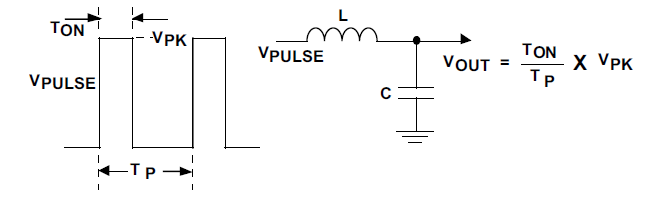
\includegraphics[keepaspectratio=true, scale=0.8]{imagens/PWM_sample.png}}
\captionof{figure}{Exemplo de uma saída PWM. Fonte: \cite{ti_whitepaper}}
\label{PWM_sample_fig}
\end{minipage}

A saída na forma de onda quadrada é filtrada e fornece uma tensão de saída DC igual ao valor da tensão de pico $V_{pk}$ multiplicada pelo \textit{Duty Cycle}, que é a razão entre o período ligado e o período local. Esta relação explica como a tensão de saída conversor pode ser diretamente controlada apenas alterando o Duty Cycle.  

\subsection*{Topologia SEPIC}
O nome SEPIC (\textit{Single-Ended Primary Inductance Converter}), ou, em tradução livre, Conversor com Indutância Simples no Primário é um conversor capaz de converter uma tensão DC de entrada para uma tensão DC maior ou menor, porém sem que ocorra inversão de polaridade. Essa característica traz uma versatilidade muito boa para essa topologia de conversor, uma vez que a inversão de polaridade costuma ser indesejada em muito projetos.  Para essa topologia, como a utilizaremos bastante mais adiante, vamos realizar a demonstração da relação entre as tensões de entrada e saída.   

\noindent
\begin{minipage}{\linewidth}
\makebox[\linewidth]{
    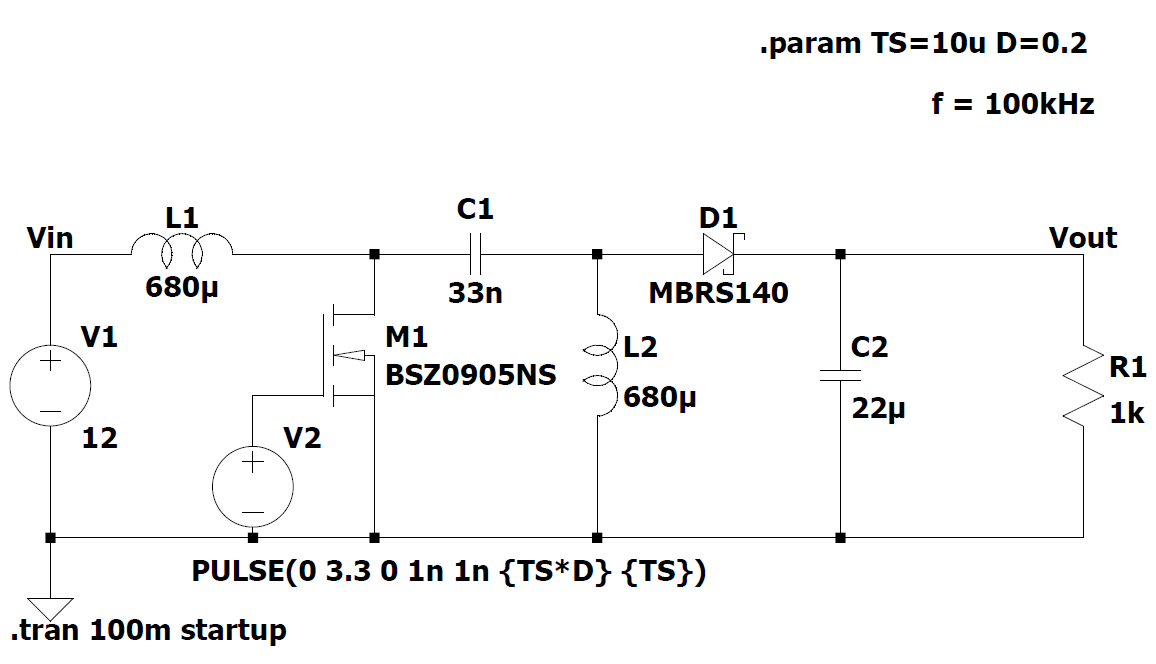
\includegraphics[keepaspectratio=true, scale=0.5]{imagens/SEPIC_full.png}}
\captionof{figure}{Exemplo da topologia SEPIC}
\label{sepic_topology_sample}
\end{minipage}

\noindent
\begin{minipage}{\linewidth}
\makebox[\linewidth]{
    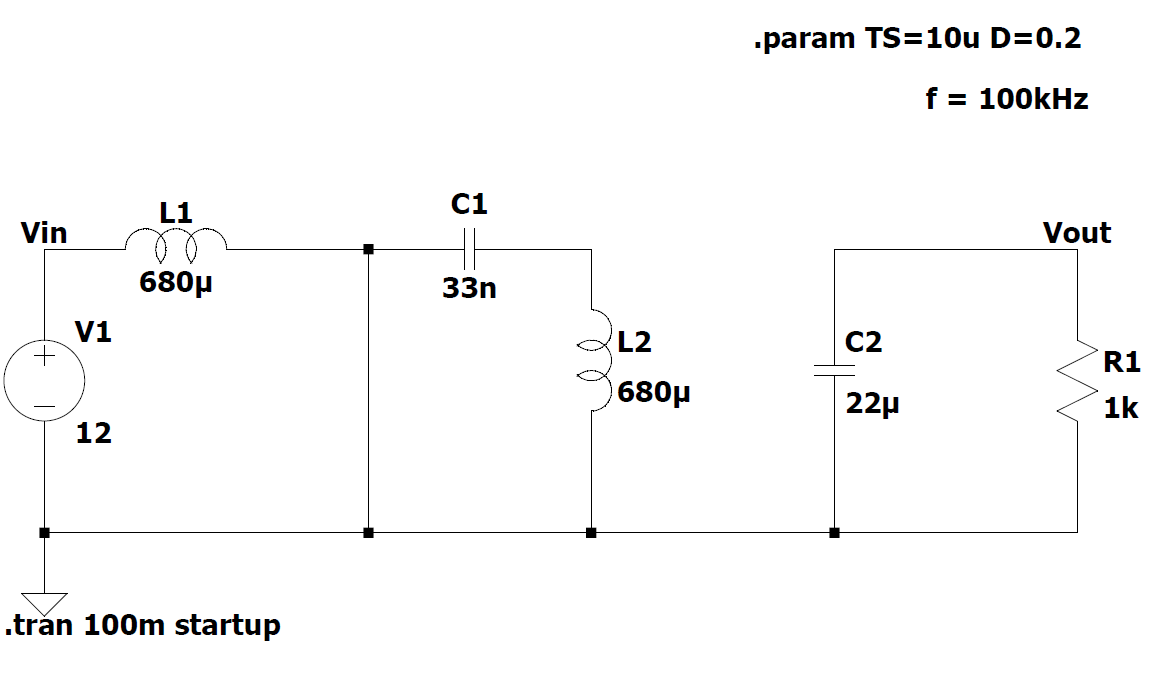
\includegraphics[keepaspectratio=true, scale=0.5]{imagens/SEPIC_closed.png}}
\captionof{figure}{Topologia SEPIC com a chave fechada e o diodo em polarização reversa}
\label{sepic_topology_closed_sample}
\end{minipage}

\noindent
\begin{minipage}{\linewidth}
\makebox[\linewidth]{
    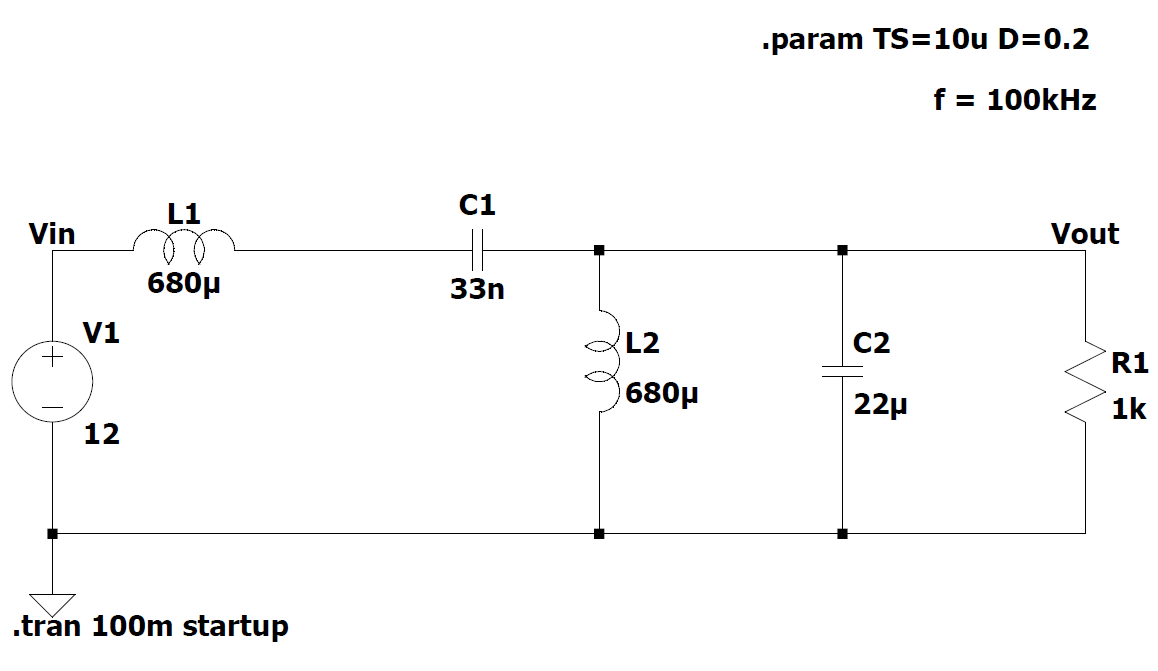
\includegraphics[keepaspectratio=true, scale=0.5]{imagens/SEPIC_open.png}}
\captionof{figure}{Topologia SEPIC com a chave aberta e o diodo em polarização direta}
\label{sepic_topology_open_sample}
\end{minipage}

\paragraph{}
Para a demonstração abaixo, são colocadas as seguintes premissas:
\begin{enumerate}
    \item os indutores são grandes o suficiente para que as correntes sejam constantes;
    \item os capacitores são grandes o suficiente para que as tensões sejam constantes;
    \item o circuito está operando no estado estável, o que significa que a formas de onda de tensão e corrente são períodicas;
    \item para um \textit{Duty Cycle D}, a chave fica fechada por \textit{$DT$} e aberta por \textit{$(1 - D)T$};
    \item a chave e o diodo são ideais.
\end{enumerate}

Aplicando a Lei de \textit{Kirchoff} no laço $V_{1}$, $L_{1}$, $C_{1}$, $L_{2}$:
\begin{equation}
    - V_{1} + V_{L1} + V_{C1} - V_{L2} = 0
\end{equation}

Considerando a tensões médias nos indutores:
\begin{equation}
    \begin{split}
        - V_{1} + 0 + V_{C1} - 0 = 0 \\ V_{C1} = V_{1}
    \end{split}
    \label{sepic_eq_1}
\end{equation}

Quando a chave está fechada e o diodo em polarização reversa, conforme na figura \ref{sepic_topology_closed_sample}. A tensão em $L_{1}$ pelo período \textit{DT} é:
\begin{equation}
    V_{L1} = V_{S}
\end{equation}

Quando a chave está aberta e o diodo em polarização direta, conforme na figura \ref{sepic_topology_open_sample}. A Lei de \textit{Kirchoff} no laço mais externo nos entrega:
\begin{equation}
    -V_{1} + V_{L1} + V_{C1} + V_{R1} = 0
\end{equation}

Substituindo a relação \ref{sepic_eq_1}:
\begin{equation}
    \begin{split}
        -V_{1} + V_{L1} + V_{1} + V_{R1} = 0 \\
        V_{L1} = - V_{R1}
    \end{split}
    \label{sepic_eq_2}
\end{equation}

Expandindo a equação considerando os períodos da chave aberta e chave fechada:
\begin{equation}
    \begin{split}
        V_{L1 (SW CLOSED)} (DT) + V_{L1 (SW OPEN)} (1-D)T = 0\\
        V_{1}(DT) - V_{R1}(1-D)T = 0\\
        V_{R1} = V_{1} (\frac{D}{1-D})
    \end{split}
\end{equation}

Onde \textit{D} é o \textit{Duty Cycle} aplicado na chave.

\subsection*{Topologia Buck}
A topologia de conversor chaveado mais utilizada é a \textit{Buck}, utilizada para converter uma tensão DC para uma tensão DC menor e de mesma polaridade. Para essa topologia, apresenta-se apenas uma análise qualitativa, uma vez que a relação entre as tensões pode ser feita de forma analóga ao conversor SEPIC. O conversor \textit{buck} utiliza um transistor para chavear a tensão de entrada para o indutor, conforme observado no circuito abaixo:

\noindent
\begin{minipage}{\linewidth}
\makebox[\linewidth]{
    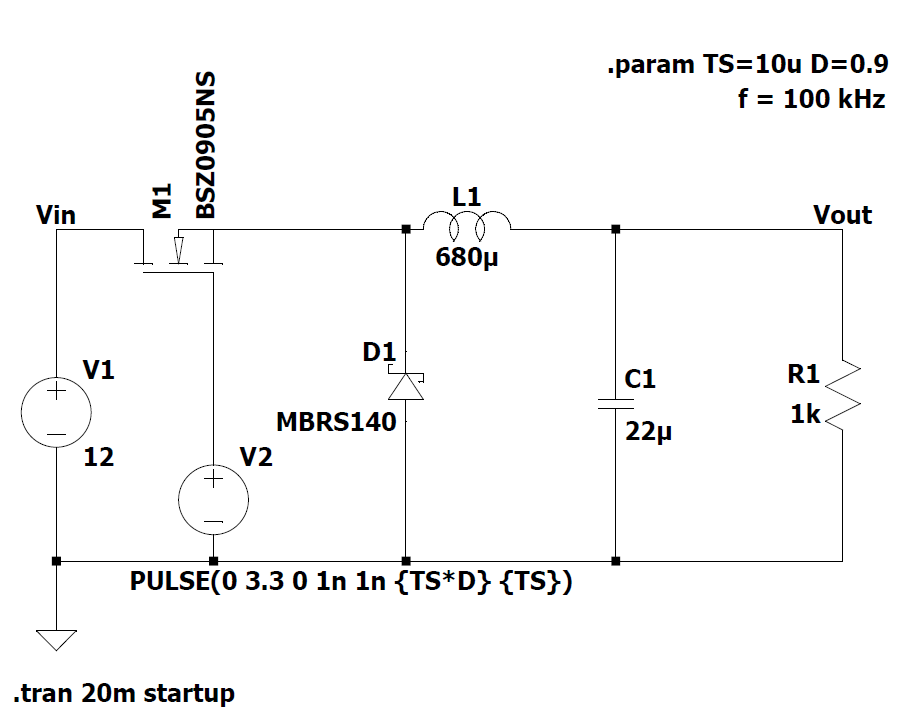
\includegraphics[keepaspectratio=true, scale=0.5]{imagens/Buck_sample.png}}
\captionof{figure}{Exemplo da topologia Buck}
\label{buck_topology_sample}
\end{minipage}

Quando a chave é ligada, a tensão de entrada é conectada com o indutor. A diferença entre as tensões da entrada e saída é forçada através do indutor, fazendo com que a corrente passando por ele aumente. Portanto, enquanto a chave estiver ligada, a corrente passa pela carga e pelo capacitor de saída, que está sendo carregado durante o período. Quando a chave é desligada, a tensão aplicada no indutor some, entretanto, como a corrente de um indutor não pode mudar instantaneamente, caso contrário estaríamos violando a Lei da Indutância\footnote{Pela Lei da Indutância, seria necessário uma tensão infinita para interromper a corrente passando um indutor de forma instântanea}, a tensão através do indutor será ajustada para manter a corrente constante.

A extremidade de entrada do indutor é forçada pela tensão negativa devido à diminuição da corrente, eventualmente colocando o diodo no estado de condução, a partir desse momento a corrente do indutor passa pela carga e volta atráves do diodo. Ainda durante o período de chave desligada, o capacitor de saída se descarrega na carga, contribuindo com a corrente total que é fornecida durante o período. 


\section{MPPT - Maximum Peak Point Tracking}\label{mppt_revision}
A configuração em que o painel solar é conectado diretamente a bateria, sem o auxílio de um controlador de carga, causa uma situação de baixa eficiência, pois, nessas circunstâncias, a célula dificilmente estará operando no seu ponto ótimo, isto é, o ponto na curva I-V que entrega a máxima potência possível.

A técnica MPPT, Rastreamento do Ponto de Máxima Potência, em tradução livre, é usada para extrair a máxima potência de um painel solar e transferi-la para a carga. Para atingir esse objetivo, um conversor DC/DC é utilizado com interface entre a carga e o painel solar, de tal forma que ao alterar o \textit{duty cycle} a impedância vista pela fonte varia para combinar com o ponto de máxima potência e assim transferir a máxima potência para a carga. A seguir, faremos uma comparação entre dois algoritmos bastante populares para implementação da técnica MPPT \cite{mppt_comparison}.

\subsection*{Algoritmo: Pertuba e Observa}
O Pertuba e Observa, também conhecido como P\&O, é um algoritmo iterativo que analisa a potência do circuito em tempos discretos e com essas informações toma uma decisão de qual ajuste deve ser feito no circuito. 

\noindent
\begin{minipage}{\linewidth}
\makebox[\linewidth]{
    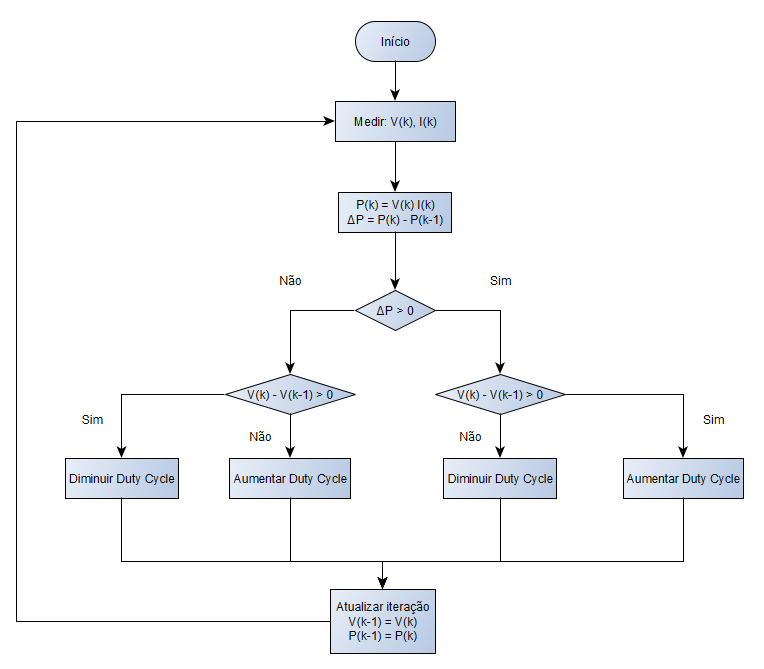
\includegraphics[keepaspectratio=true, scale=0.5]{imagens/P&O_flux.png}}
\captionof{figure}{Fluxograma para o algoritmo Perturba e Observa}
\label{PO_flux_fig}
\end{minipage}

No inicio do ciclo, o primeiro passo é aferir a tensão e corrente na carga. Com esses dados, calcula-se o $\Delta$P (variação da potência) entre a iteração atual e a anterior, em seguida, avalia-se se a tensão é maior ou menor do que a observada na iteração anterior. Com todos esses dados adquiridos, surgem quatro ramos de decisão:
\begin{enumerate}
    \item A potência aumentou e a tensão aumentou: aumentar o \textit{Duty Cycle} no conversor 
    \item A potência aumentou e a tensão diminuiu: diminuir o \textit{Duty Cycle} no conversor
    \item A potência diminuiu e a tensão aumentou: diminuir o \textit{Duty Cycle} no conversor
    \item A potência diminuiu e a tensão diminuiu: aumentar o \textit{Duty Cycle} no conversor
\end{enumerate}

Após fazer as correções no conversor os valores dessa iteração são salvos para serem usado posteriormente como comparação com a iteração seguinte. O algoritmo P e O é amplamente utilizado devido a simplicidade de implementação e boa eficiência. Um ponto desfavorável desse algoritmo é que ele não consegue atingir uma estabilidade quando próximo do ponto de máxima potência, uma vez que ele sempre estará avaliando e tentando ajustar o circuito.

\subsection*{Algoritmo: Condutância Incremental}

O algoritmo da Condutância Incremental (CI) corrige um dos problemas do Pertuba e Observa que é a estabilidade quando se atinge o ponto de máxima potência, o algoritmo é capaz de determinar que esse ponto foi atingindo e não mais alterar a configuração de operação. Além disso, ele é capaz de reagir com melhor precisão as mudanças abruptas de irradiação, a desvantagem em relação ao algoritmo P\&O é com a sua maior complexidade de implementação. Abaixo, segue o fluxograma e a explicação do algoritmo CI.

\noindent
\begin{minipage}{\linewidth}
\makebox[\linewidth]{
    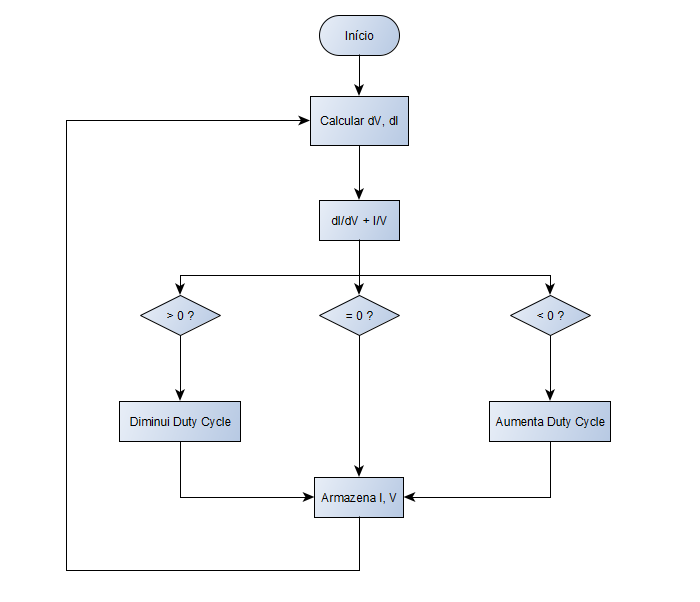
\includegraphics[keepaspectratio=true, scale=0.5]{imagens/CI_flux.png}}
\captionof{figure}{Fluxograma para o algoritmo Condutância Incremental}
\label{CI_flux_fig}
\end{minipage}

Se a condição de equilibrio não for encontrada, a direção em que o ponto de operação MPPT deve ser perturbado, realizando a alteração no $\frac{dI}{dV}$ e $\frac{-I}{V}$. Essa relação é derivada do fato de que $\frac{dP}{dV}$ é negativo quando o MPPT está à direita do ponto de máxima potência e positivo quando está à esquerda.

